\par Dans la présente Section, on va découvrir ce qui a été concrètement réaliser durant le stage, ainsi que tout les outils utilisés pour mener a bien les différents projets. J'essayerais, par la suite, de présenter un bilan général des six mois de stage.  

\begingroup
    \let\clearpage\relax
    \chapter{Environnement technique et outils technologiques}
\endgroup
\section{Outils communs}
\par Dans la présente section, je présenterais tout les outils commun a tout les projets, notamment les outils fonctionnels (outils de planification \dots) ainsi que les outils pour vérifier la qualité du code et déploiement des applications. 
\subsection{La suite Atlassian}
\par Atlassian est un éditeur de logiciels, basé en Australie, qui développe des produits pour la gestion de développement et de projets. Ses logiciels les plus connus sont Jira, Confluence, Bamboo, Bitbucket et Trello. Une grande parte de la suite Atlassian est payante.
\par Pour nos projets, j'ai pu utiliser JIRA et Confluence.

\subsubsection{Jira}
\par JIRA est un « issue tracker ». On pourrait traduire : un « Gestionnaire de demande ». Cette définition donne une idée du potentiel de l’outil mais reste néanmoins imparfaite parce que le terme anglais « Issue » fait référence à quelque chose de beaucoup plus générique. Une « Issue » est en fait un objet, sujet, ou situation, susceptible d’être traité. Il peut donc s’agir de bug, d’anomalies, d’incidents, de demandes d’intervention, mais aussi de la multitude des taches anodines qui font le quotidien de chacun d’entre nous. JIRA est un outil de suivi d’activités.
\clearpage
\par En pratique les cas d’utilisation de JIRA les plus souvent rencontrés sont les suivants :
\begin{itemize}
    \item La gestion du support et des activités de développement logiciel
    \item Le suivi des anomalies
    \item Le suivi d’activité
    \item La gestion de Centres de services
\end{itemize}
\begin{figure}[ht]
    \centering
    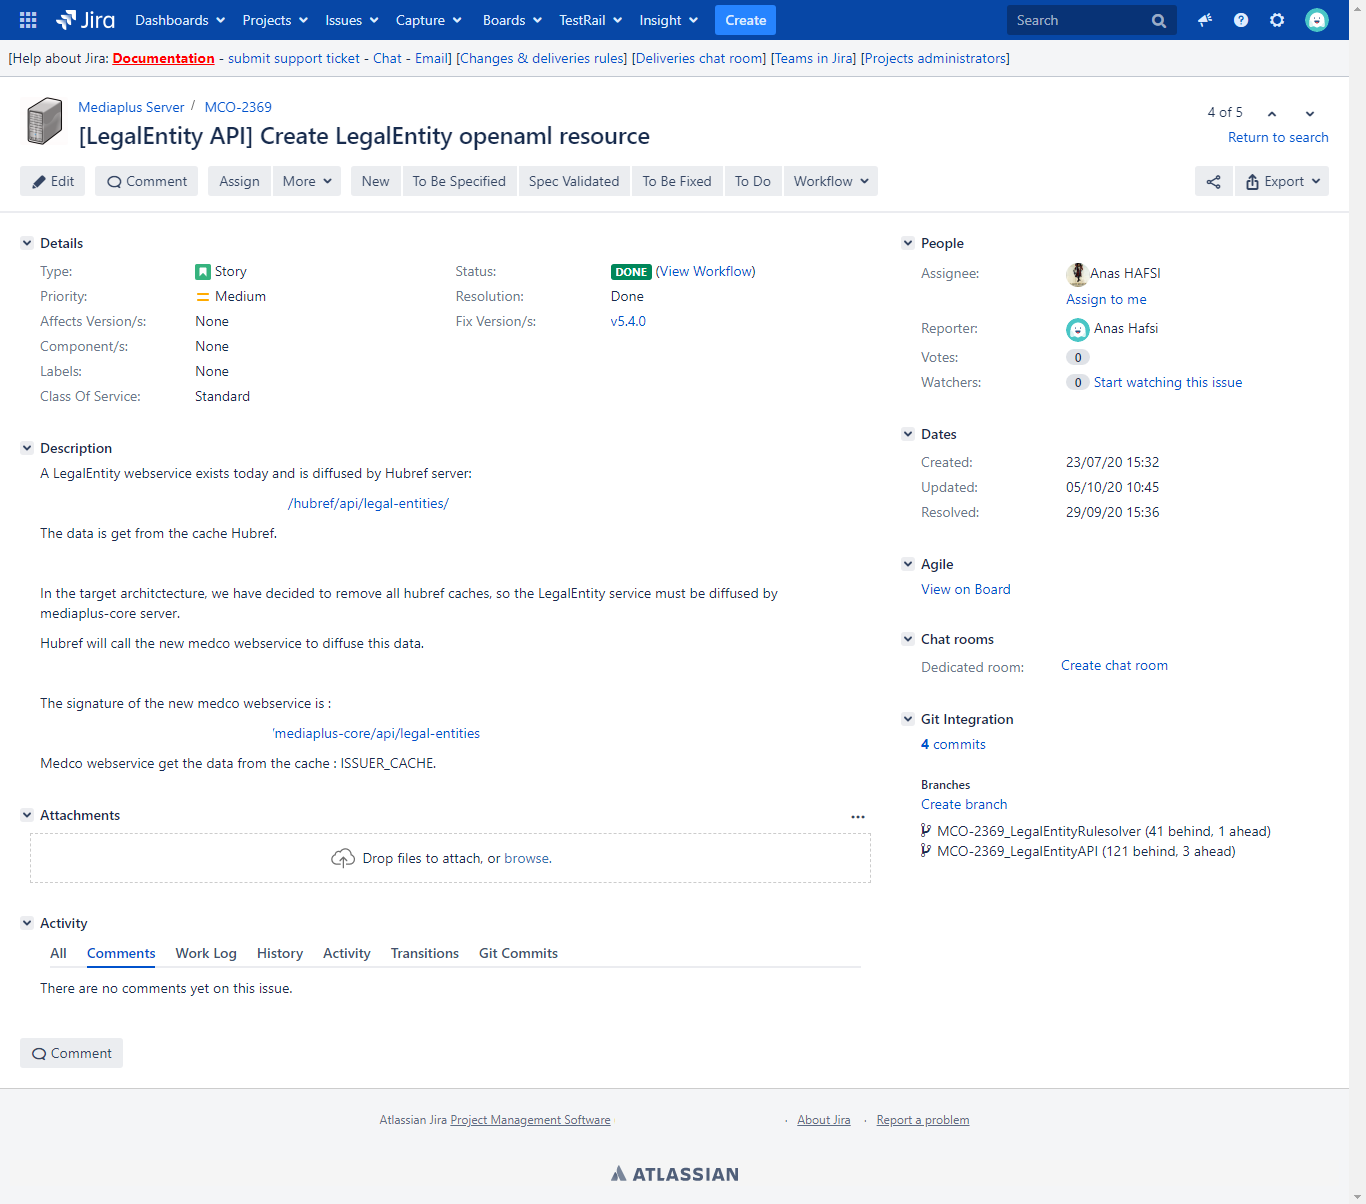
\includegraphics[width=\columnwidth]{img/JIRA MCO-2369.png}
    \caption{Ticket Jira MediaPlus Core}
    \label{fig:JiraMedco}
\end{figure}

\par Les "Issue" Jira sont nommée des tickets (exemple figure \ref{fig:JiraMedco}). l'ensemble de tickets appartenant au même sprint Agile sont rassemblé dans un "board JIRA" (exemple figure \ref{fig:JiraAlto}).
\clearpage
\begin{figure}[ht]
    \centering
    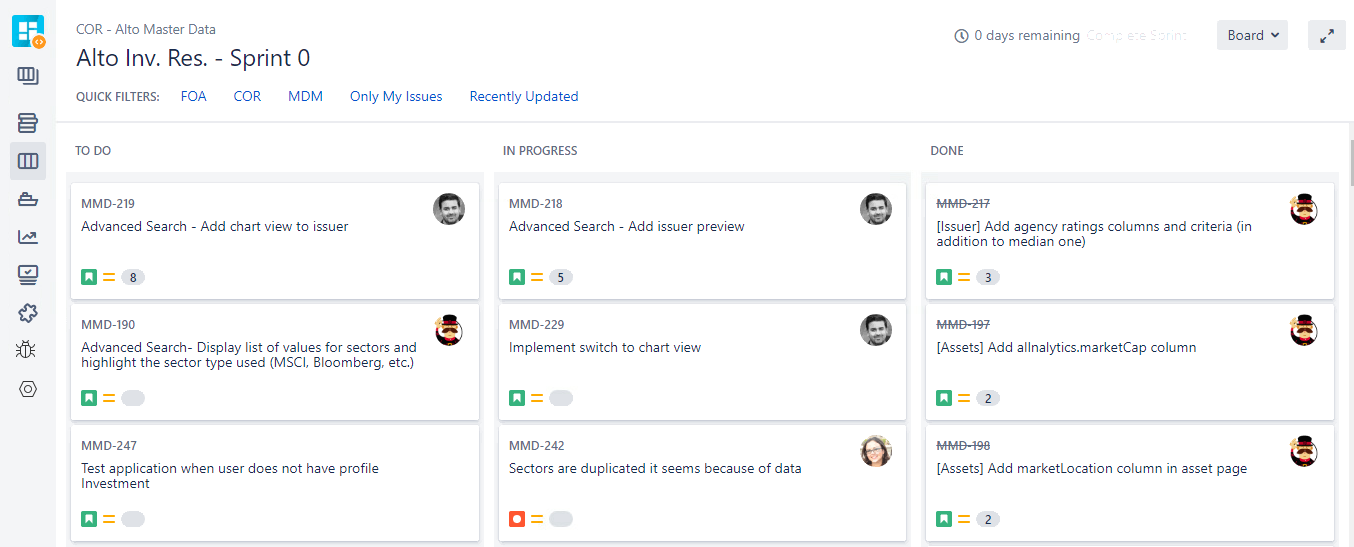
\includegraphics[width=\columnwidth]{img/Sprint Alto.png}
    \caption{Jira Board pour un sprint Alto Investment Research}
    \label{fig:JiraAlto}
\end{figure}
\subsubsection{Confluence}
\par Créez, collaborez et organisez tout votre travail à un seul et même endroit. Confluence est un espace de travail en équipe où la connaissance et la collaboration se rejoignent. Les pages dynamiques permettent à votre équipe de disposer d'un endroit pour créer, capturer et collaborer sur le projet ou l'idée de votre choix. Grâce aux espaces, votre équipe peut structurer, organiser et partager les tâches, afin que chacun de ses membres dispose d'une visibilité sur les connaissances institutionnelles ainsi que d'un accès aux informations nécessaires pour optimiser le travail.
\par Confluence s'adresse aux équipes de toute taille et de tout type. Qu'il s'agisse d'équipes ayant des projets stratégiques aux enjeux élevés, qui nécessitent de la rigueur dans leurs pratiques, ou d'équipes à la recherche d'un espace pour développer une culture d'équipe et interagir les unes avec les autres de manière plus ouverte et plus authentique. Grâce à Confluence, votre équipe peut prendre des décisions rapides, gagner en alignement et accomplir plus ensemble. {\tiny source: Atlassian documentation}
\par La figure \ref{fig:conf} represente un espace confluence.
\begin{figure}[ht]
    \centering
    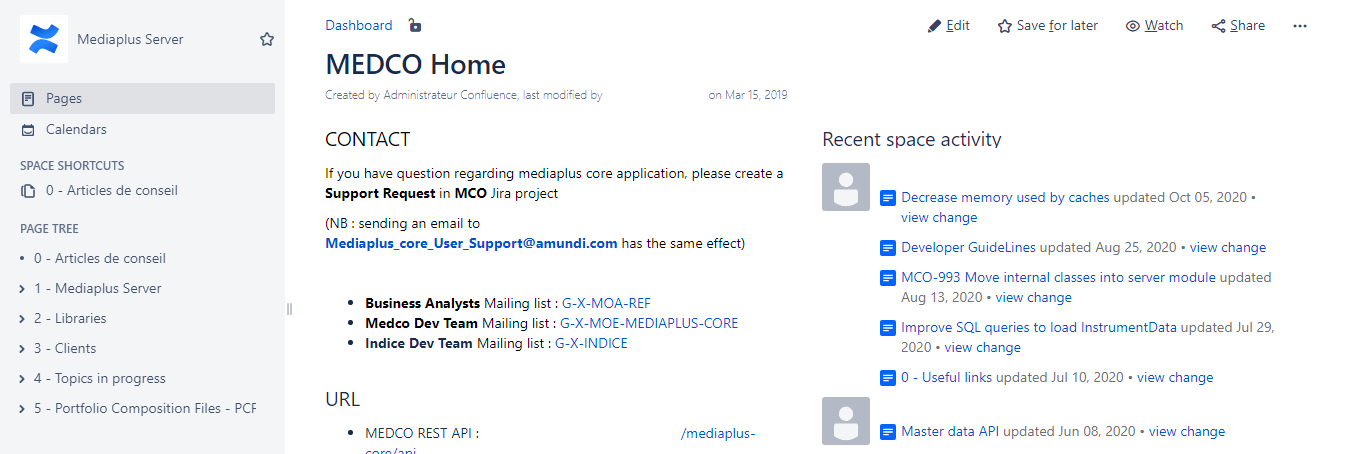
\includegraphics[width=\columnwidth]{img/ConfMedco.png}
    \caption{Espace Confluence MediaPlus-Core}
    \label{fig:conf}
\end{figure}

\subsection{Gitlab} 
\par GitLab est une plateforme de développement collaborative qui couvre l’ensemble des étapes du DevOps. Se basant sur les fonctionnalités du logiciel Git, elle permet de réaliser des dépôts et de gérer les versions de vos codes sources. Son usage est particulièrement indiqué pour les développeurs qui souhaitent disposer d’un outil réactif et accessible.
\par Comparé au autres logiciels de gestion de version, GitLab propose des options pour le moins pratiques :
\begin{itemize}
    \item Test de logiciels
    \item Configuration
    \item Monitoring
    \item Sécurité applicative
    \item Intégration et déploiement continus, etc\dots
\end{itemize}
\par Pour accompagner Gitlab on utilise SourceTree, un logiciel propriétaire du groupe Atlassian. C'est un logiciel front permettant de plus visualiser les branches git : un client frontend pour GitLab.
\begin{figure}[ht]
    \centering
    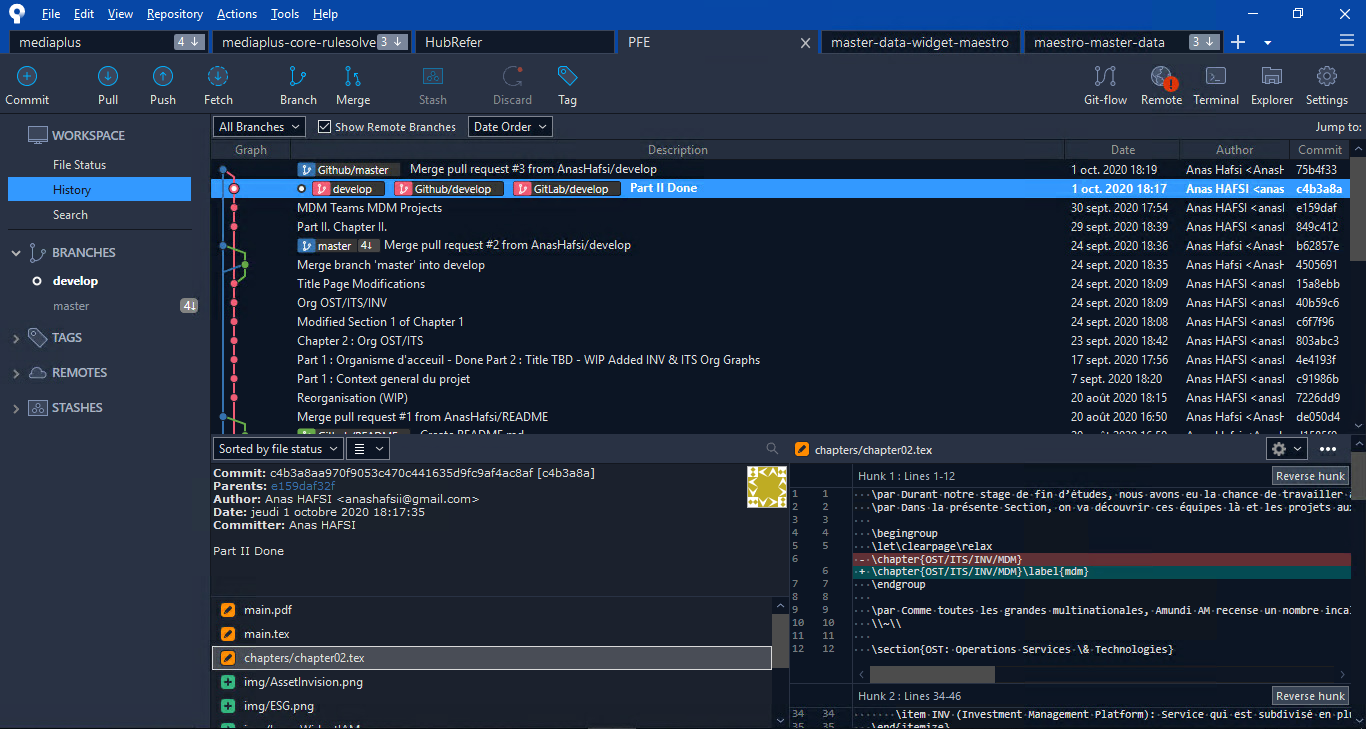
\includegraphics[width=\columnwidth]{img/sourcetree.png}
    \caption{SourceTree: interface pour la branche git contenant mon Rapport de stage}
\end{figure}
\clearpage
\subsection{Jenkins}
\par Jenkins est outil de compilation en continu des sources sur le serveur distant  Git. Il permet le lancement de processus automatiques : Compilation à  récurrence fixe, affichage de la dégradation de la qualité du code, lance les  tests unitaires des projets. Cet outil nécessite énormément de configuration  pour pour commencer à être productif. 
\par Jenkins contient une série de jobs génériques qui ont une utilité particulière. Il  nous est impossible de créer nos propres jobs génériques faute de droits (en  général de besoin. Les jobs génériques couvrent quasiment tous les cas)
\begin{figure}[ht]
    \centering
    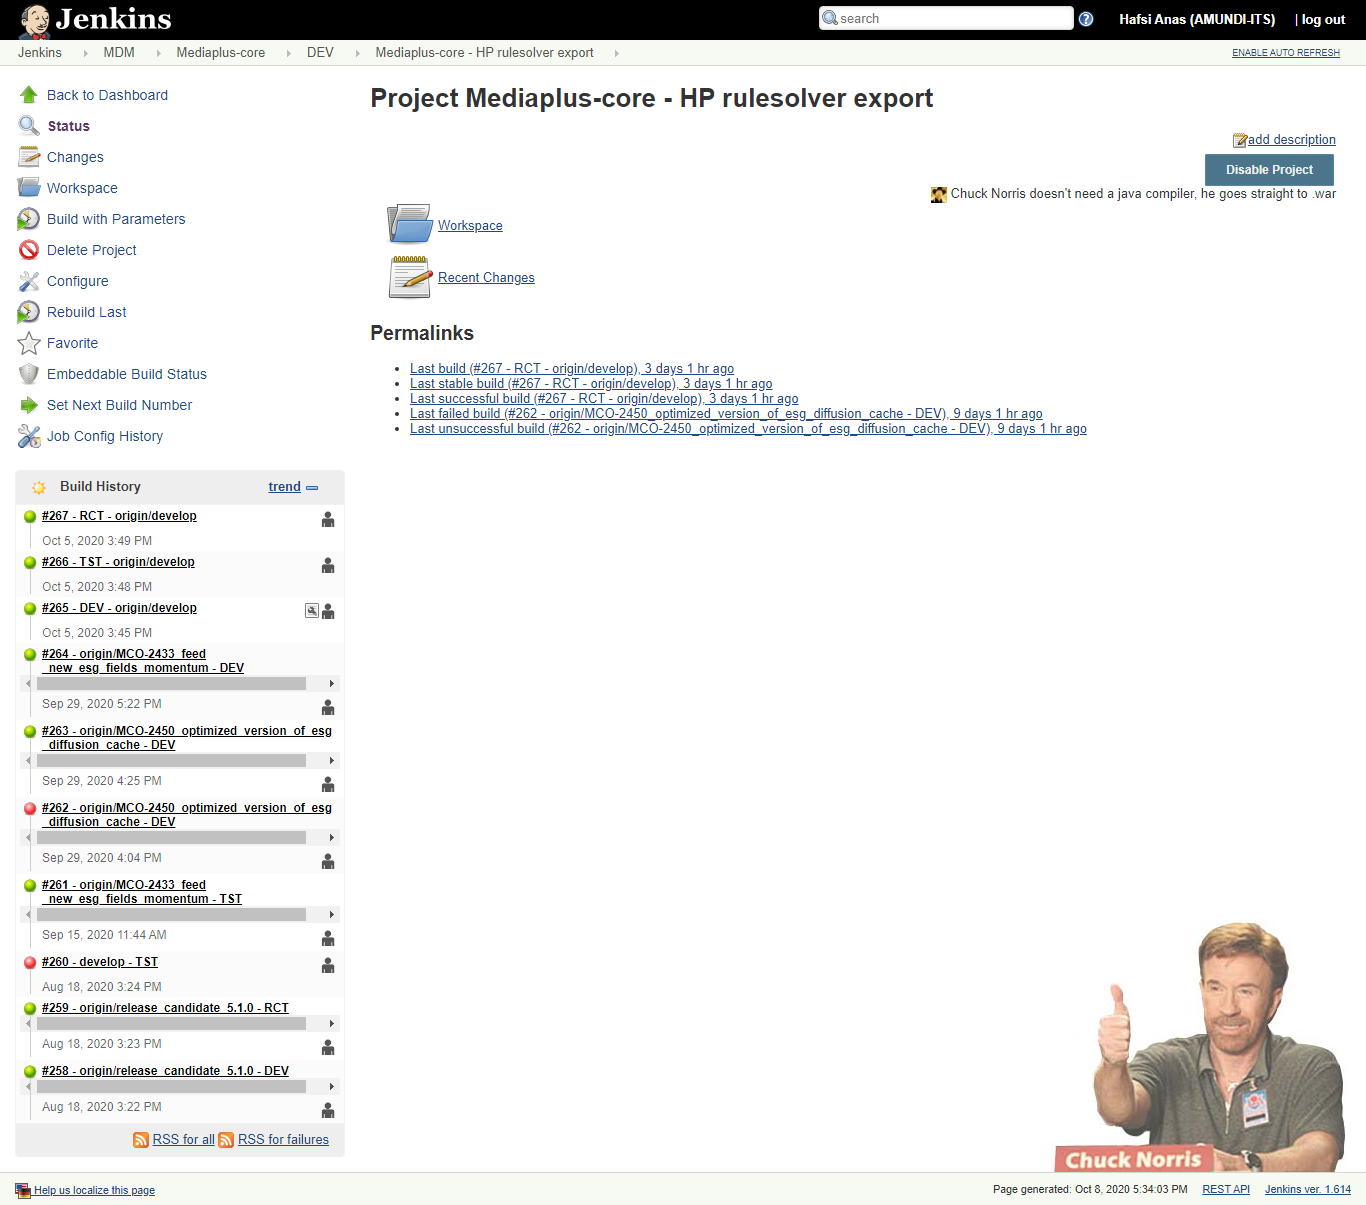
\includegraphics[width=\columnwidth]{img/jenkins.png}
    \caption{Interface Jenkins pour une branche MediaPlus-Core}
\end{figure}
\clearpage
\section{Outils MediaPlus Core}
\par Durant la présente section, on présentera les différents outils technique qu'on a utilisé dans la réalisation des différents tickets JIRA.
\par On va retrouver par exemple des logiciels qui nous permettrons d'accéder au différentes bases de données, des logiciels pour pouvoir faire du monitoring sur l'application MediaPlus-Core des différents environnements (DEV, TEST, RCT, PPR, PROD), pour gérer les differents caches disponibles sur l'application mais aussi pour pouvoir récupérer les différentes données.

\subsection{SQuirreL}
\par SQuirreL SQL Client est une interface graphique open source qui vous permet de visualiser la structure de bases de données conformes JDBC, charger les données dans des tables, ou encore lancer des requêtes SQL.
\par Développé en JAVA, SQuirreL SQL Client est fourni avec une documentation détaillée pour guider au mieux parmi les nombreuses fonctionnalités proposées.
\begin{figure}[ht]
    \centering
    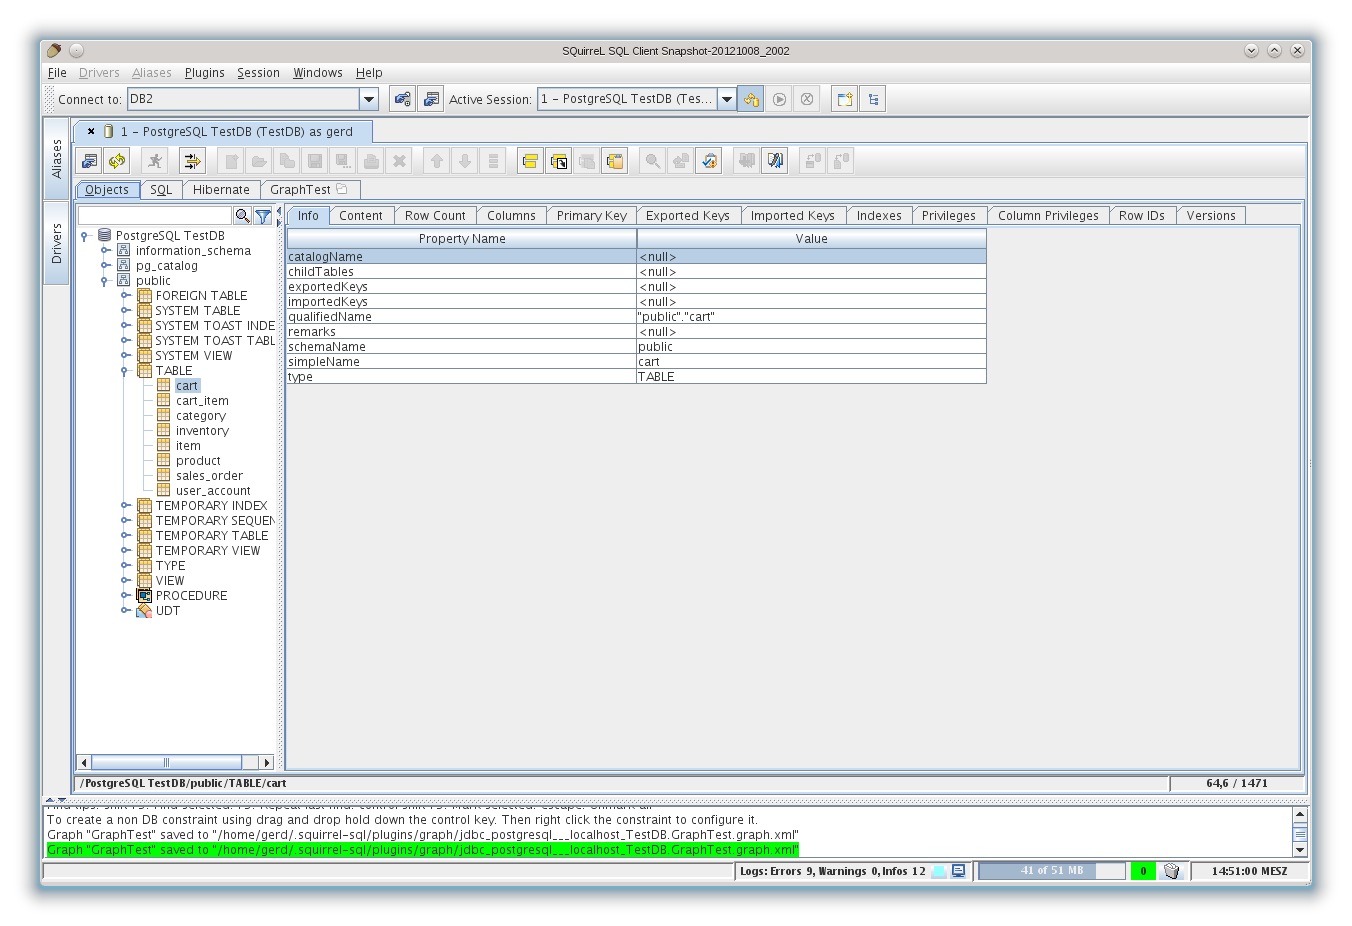
\includegraphics[width=\columnwidth]{img/sqrl.png}
    \caption{Interface SQuirreL}
\end{figure}
\subsection{Server Admin}
\par Comme le nom l'indique, cette application front est considéré comme un administrateur de tout les serveur/applications Amundi-ITS (Exemple: Refgt, Alto, Medco\dots).
\par Cette application, developpé pendant les premieres années d'activité d'Amundi AM (pour des raisons de confidentialité je ne citerais pas la date), regroupe trois fonctions majeurs, le monitoring, la gestion et l'affichage de donnée.
\begin{itemize}
    \item Monitoring: Permet de surveiller et contrôler le serveur MediaPlus-Core.
    \item Gestion: Permet de contrôler les differents caches MediaPlus-Core (supprimer, recharger, décharger, serialiser, deserialiser).
    \item Affichage: Afficher les differentes données diffusé par les Ejb MediaPlus-Core.
\end{itemize}
\par La figure \ref{fig:serveradmin} représente l'interface de la partie MediaPlus-core dans ServerAdmin. Des champs ont été caché pour des raisons de confidentialité.
\begin{figure}[ht]
    \centering
    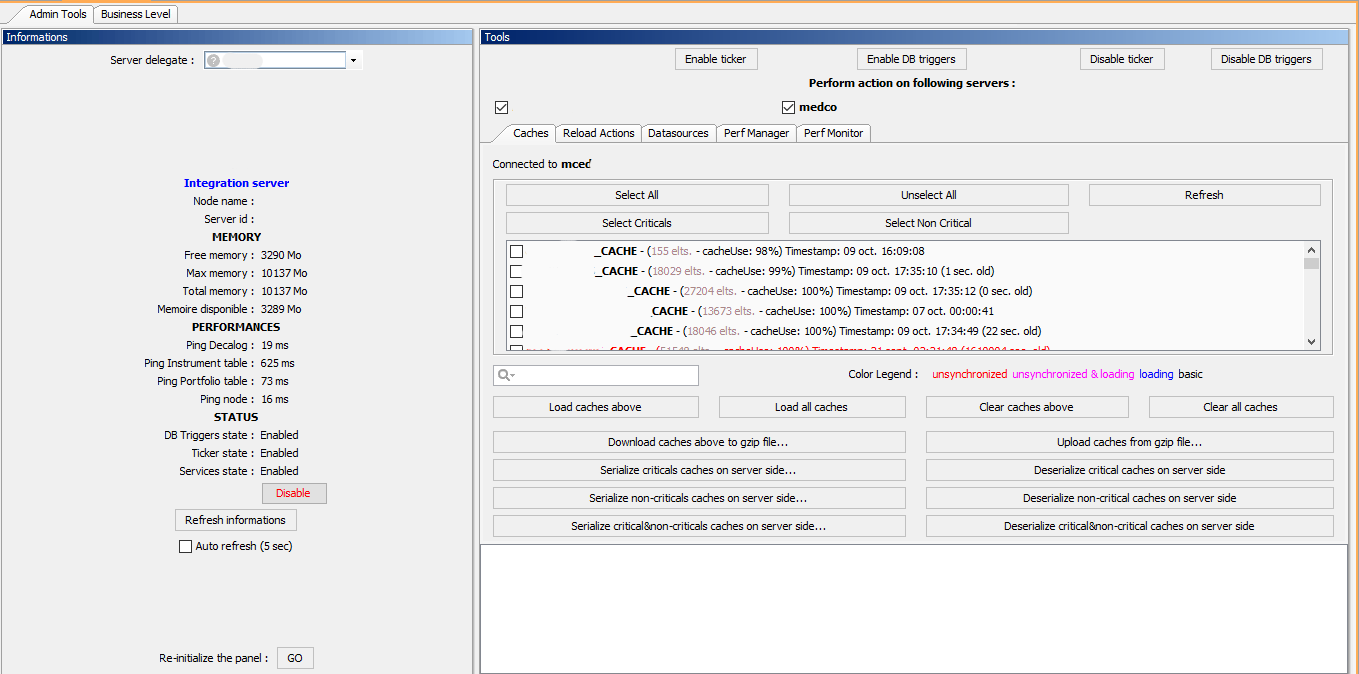
\includegraphics[width=\columnwidth]{img/serveradmin.png}
    \caption{Server Admin}
    \label{fig:serveradmin}
\end{figure}

\subsection{Apache Maven}
\par Apache Maven (couramment appelé Maven) est un outil de gestion et d'automatisation de production des projets logiciels Java en général et Java EE en particulier. Il est utilisé pour automatiser l'intégration continue lors d'un développement de logiciel. Maven est géré par l'organisation Apache Software Foundation. L'outil était précédemment une branche de l'organisation Jakarta Project.
\par L'objectif recherché est de produire un logiciel à partir de ses sources, en optimisant les tâches réalisées à cette fin et en garantissant le bon ordre de fabrication. Il peut se comparer au système make sous Unix ou à l'outil Ant.
\par Maven utilise un paradigme connu sous le nom de Project Object Model (POM) afin de décrire un projet logiciel, ses dépendances avec des modules externes et l'ordre à suivre pour sa production. Il est livré avec un grand nombre de tâches pré-définies, comme la compilation de code Java ou encore sa modularisation.
\par Un élément clé et relativement spécifique de Maven est son aptitude à fonctionner en réseau. Une des motivations historiques de cet outil est de fournir un moyen de synchroniser des projets indépendants : publication standardisée d'information, distribution automatique de modules jar. Ainsi en version de base, Maven peut dynamiquement télécharger du matériel à partir des dépôts logiciels connus. Il propose ainsi la synchronisation transparente de modules nécessaires.
\par L'architecture Maven du projet est disponible dans la figure \ref{fig:mavenarch}. \\
\begin{figure}[ht]
    \begin{lstlisting}
    MediaPlus-Core
    |-- pom.xml
    `-- mediaplus-core-batch
        |-- pom.xml
    `-- mediaplus-core-dist
        |-- pom.xml
    `-- mediaplus-core-ejb
        |-- pom.xml
    `-- mediaplus-core-ejb-server
        |-- pom.xml
    `-- mediaplus-core-server
        |-- pom.xml
    `-- mediaplus-core-to-openaml
        |-- pom.xml
    `-- mediaplus-core-ws
        |-- pom.xml
    `-- mediaplus-core-ws-api
        |-- pom.xml
    `-- mediaplus-core-ws-doc
        |-- pom.xml
    `-- launchers
        `-- local
    `-- doc
    \end{lstlisting}
    \caption{Archetype Maven}
    \label{fig:mavenarch}
\end{figure}
\clearpage
\section{Outils Alto Investment Research}
\par En ce qui concerne Alto Investment Research, on a utilisé, en plus des outils communs, InVision et la documentation Maestro.
\subsection{InVisionApp}
\par InVision est une application accessible par navigateur Internet (SaaS) qui vous permet de présenter vos visuels à même le navigateur du client qui verra exactement de quoi son projet a l’air sur son écran. On évite ainsi toutes les questions et commentaires du type « C’est beau comme ça, mais ça va avoir l’air de quoi dans mon navigateur? » ou encore « Ça a l’air petit dans votre PDF ». Les JPG que vous téléversez dans l’application sont affichés à 100\% de leur dimension et centrés dans l’écran. Il est toutefois possible de jouer avec les paramètres si votre image doit être alignée sur un côté. De plus, InVision met à votre disposition des gabarits de base pour mobile et tablette.
\par Dans la version pro d’InVision (La version Pro utilisé par Amundi AM), il est possible de gérer plusieurs projets en même temps. Chaque projet possède sa propre adresse URL aléatoire. Ainsi, un client ne pourra pas tomber par hasard sur le projet d’un autre client.
\par Les designers de l'équipe "ITS/INV/EAX Entreprise Architecture \& UX Design" réalisent les maquettes (exemple: figure \ref{fig:invision}) sur InVision, et à travers les MOE on récupère les écrans a développer pour réaliser un résultat proche de celui des EAX.
\clearpage
\begin{figure}[ht]
    \centering
    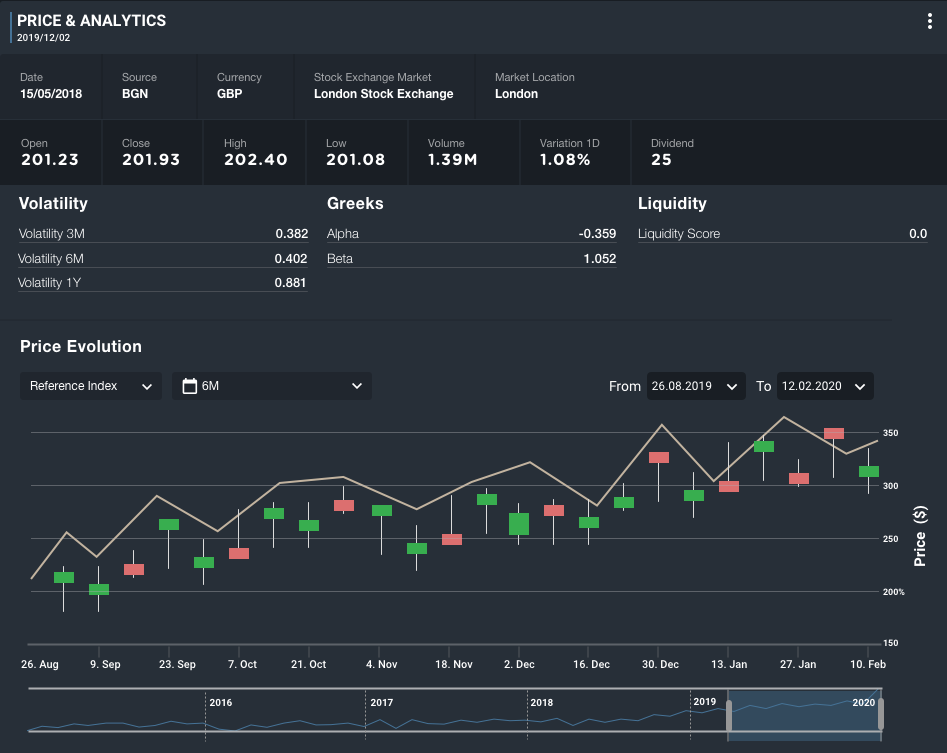
\includegraphics[width=\columnwidth]{img/AssetInvision.png}
    \caption{Exemple d'une maquette ALTO sur InVision}
    \label{fig:invision}
\end{figure} 

\subsection{Documentation Maestro}
\par Comme c'est deja mentionné dans les chapitres précédents, Maestro est un framework interne Amundi AM basé sur Angular développé par l'équipe ITS/DOT/COR, inclus plusieurs surcouches unifiant toutes les applications front Amundi AM, pouvant parfois faciliter des blocs de code.
\par Pour ce ITS/DOT/COR a mis a notre disposition une documentation complete de tout les composant Maestro ajouté par le framework, ainsi que plusieurs exemples de leurs utilisations.
\begin{figure}[ht]
    \centering
    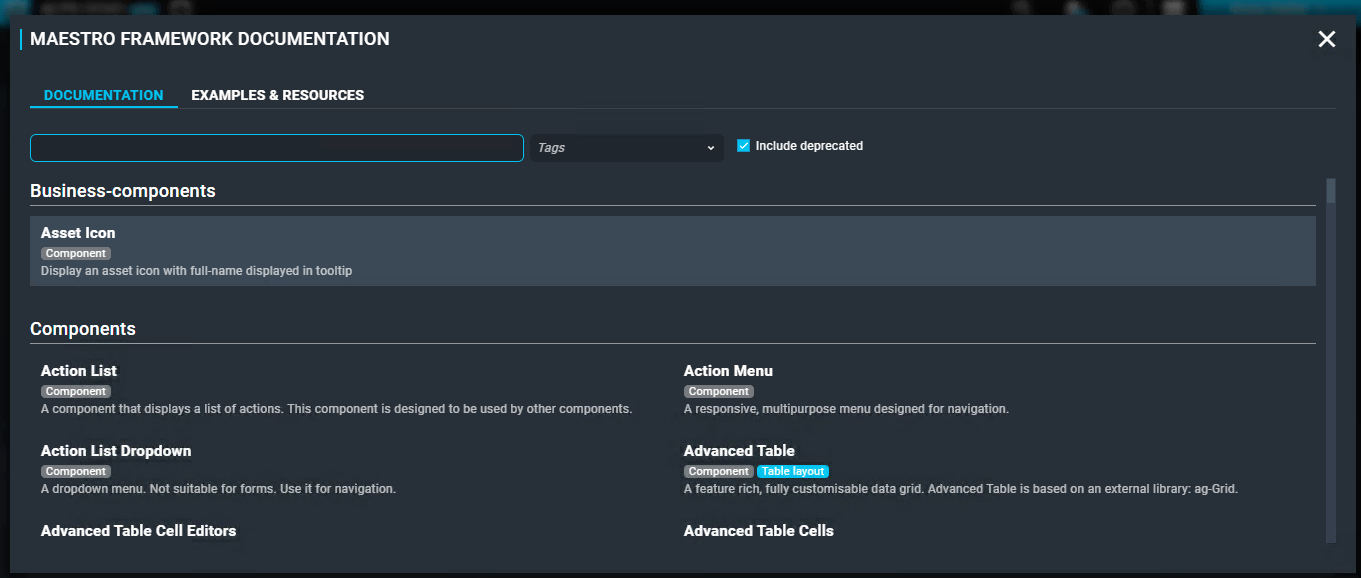
\includegraphics[width=\columnwidth]{img/maestrodocum.png}
    \caption{Exemple de la documentation Maestro}
\end{figure} 

\chapter{Travail réalisé}
\par Dans le présent chapitre on essayera de parler de tout le travail réalisé durant la période passé chez le client ainsi que l'évolution des differents projets auquel j'ai eu la chance de participer.
\section{MediaPlus-Core}
\par Durant mon stage, j'ai eu l'occasion de relisé plusieurs tickets JIRA touchant a plusieurs aspects de l'application MediaPlus-Core. J'ai pu les subdiviser en deux parties: la migration/creation de nouveaux API, et la réalisation de support requests d'autres équipes Amundi AM.
\begin{itemize}
    \item Partie API: J'ai pu créer de nouveaux API et/ou de migrer d'autres depuis le système STPML qui est déprécié au sein d'Amundi vers le system OpenAML.
    \item Support requests: Parfois des ingénieurs Amundi AM (que ça soit des développeurs ou des métiers) ont besoin d'avoir de nouveau champs diffusé par Medco oui remappé vers de nouvelles valeurs depuis les différentes bases de données. 
\end{itemize} 
\par Pour des raisons de confidentialité, je me passerais de plusieurs details (notamment noms (deuxième API) et details techniques).
\subsection{Creation d'API REST}
\par Apres avoir rejoint l'équipe Medco, J'ai pu développer (from scratch) deux nouvelles API.\\
\begin{itemize}
    \item Countries: L'API des countries est un API essentiel pour le fonctionnement d'autres API ainsi que la diffusions de plusieurs champs. En effet on peut le retrouver dans plusieurs types de données (Exemple: Currency/Devise qui est un Objet indispensable dans le domaine financier). L'API était précédemment diffusé sous format STPML, format déclaré obsolète, et donc fallait migrer et remapper les objets pour pouvoir être compatible. L'API, accessible ar l'URL medco/countries, dispose d'une fonctionnalité de recherche par identifiant, un identifiant obéissant au format ISO 3166-1 alpha-3, accessible par l'URL medco/country/ISO. L'API était doté d'un mécanisme de filtrage/recherche plus puissant qui permettait de filter tout les country par champs, le critère de filtrage était passé par url params. Par exemple je pouvait chercher tout les pays avec un iso débutant par "A" j'utilisait l'URL medco/country?ISO=A.* ou si je voulais diffuser les pays membre de la zone euro j'utilise medco/country?euroZone=true. Pour des raisons de confidentialité, le nombre de champs diffusé reste inconnu mais le mécanisme de recherche était fonctionnel pour un très grand nombre de champs (plus de 10). \\
    \item L'API qu'on nommera Entity: cet objet est un objet sensible au sein de l'écosystème Amundi AM, du coup plusieurs details seront caché. Comme pour les countries, Entity est une données très importante pour les ingénieurs Amundi AM, Seule différence est que l'API n'existait pas sous le format STPML (en tout cas pas dans le format actuel de la data), du coup il fallait coder le mapping OpenAML. En plus des caractéristique précédemment cité dans la partie API Country (recherche par champs\dots), cet API dispose d'un autre paramètres de filtrage qui nous permet d'afficher ou non des champs de data en fonction de l'Entity utilisé, on peut diffuser jusqu'à trois niveaux de data, le niveau le plus bas étant le moins complexe. \\
\end{itemize}
\subsection{Support Request}
\par Comme c'est déjà mentionné, la partie support request concernait la partie interaction avec les differents utilisateurs Amundi AM. 
\par L'équipes recevait plusieurs demandes dont on peut citer: \\
\begin{itemize}
    \item Ajout de champs: Support request le plus reçu par l'équipe. Si une équipe a besoin de diffuser un nouveau champs depuis le différentes bases de données, l'équipe Medco récupère la demande sous forme de ticket JIRA et essaye de la traiter en modifiant les ejb pour diffuser le nouveau champs.
    \item Remapping de champs: Au cas ou une équipe essaye de changer le mapping précrée, l'équipe se charge, après avoir reçu l'accord des équipe métier concerné par le champ, de le faire tout en alertant les autres équipes gérant des projets ou le champ etait utilisé. 
    \item Supression de champs: La suppression de champ est une operation rare dans l'équipe Medco. Elle occurre généralement lorsqu'un champ est obsolète ou dont la diffusion peut engendrer des erreurs dans les résultats émis par d'autres champs/services. Comme pour le remapping, l'équipe contacte les gestionnaire métier du champs, pour avoir une confirmation et procède à la suppression de champs tout en notifiant les équipes pouvant utiliser le champ en question.
\end{itemize}
\par De mon coté j'ai pu traiter les deux premiers types de support requests à savoir la creation et le remapping de champs. 
\section{Alto Investment Research}
\par Sur Alto Investment Research Referential Widgets, le but était de reproduire les designs présent sur InVision par ordre proposé par Sara Hilmi MOA Front Office, de l'équipe GES/COO/GIS/MFO.
\par Avant ma venue dans l'equipe, les widgets presents sur Alto Investment Research etait sous le format present dans la figure \ref{fig:altoV1}.
\begin{figure}[ht]
    \centering
    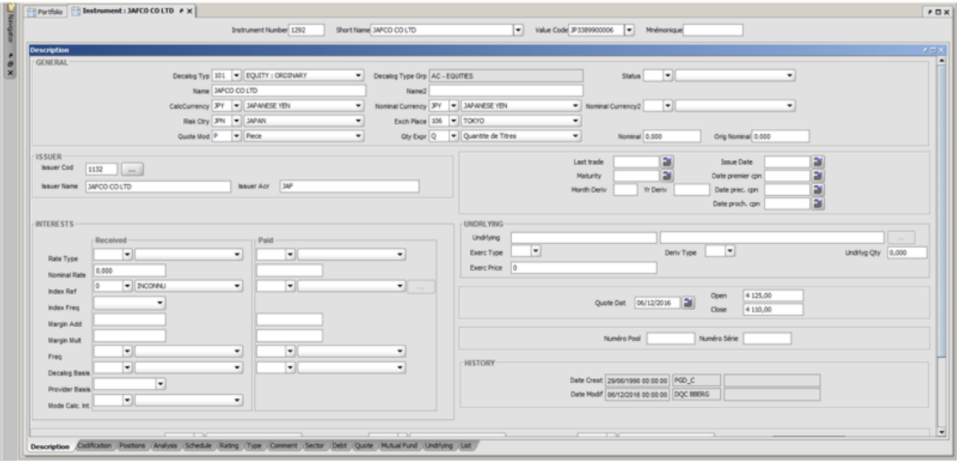
\includegraphics[width=\columnwidth]{img/ancienecrans.png}
    \caption{Anciens Écrans d'Alto Investment Research}
    \label{fig:altoV1}
\end{figure} 
\par Le but était de répliquer les écrans figurant dans la figure \ref{fig:altoInv}.
\par Le resultat realisé figure dans la figure \ref{fig:altoCurent}.
\par Plusieurs informations ont ete modifiée pour des raisons de confidentialité.
\par Mon travail consistait a réaliser les écrans (partie front), ainsi que les API Maestro pour récupérer la data depuis les differents serveurs et applications Medco (Refgt et Hubref).
\begin{figure}[ht]
    \centering
    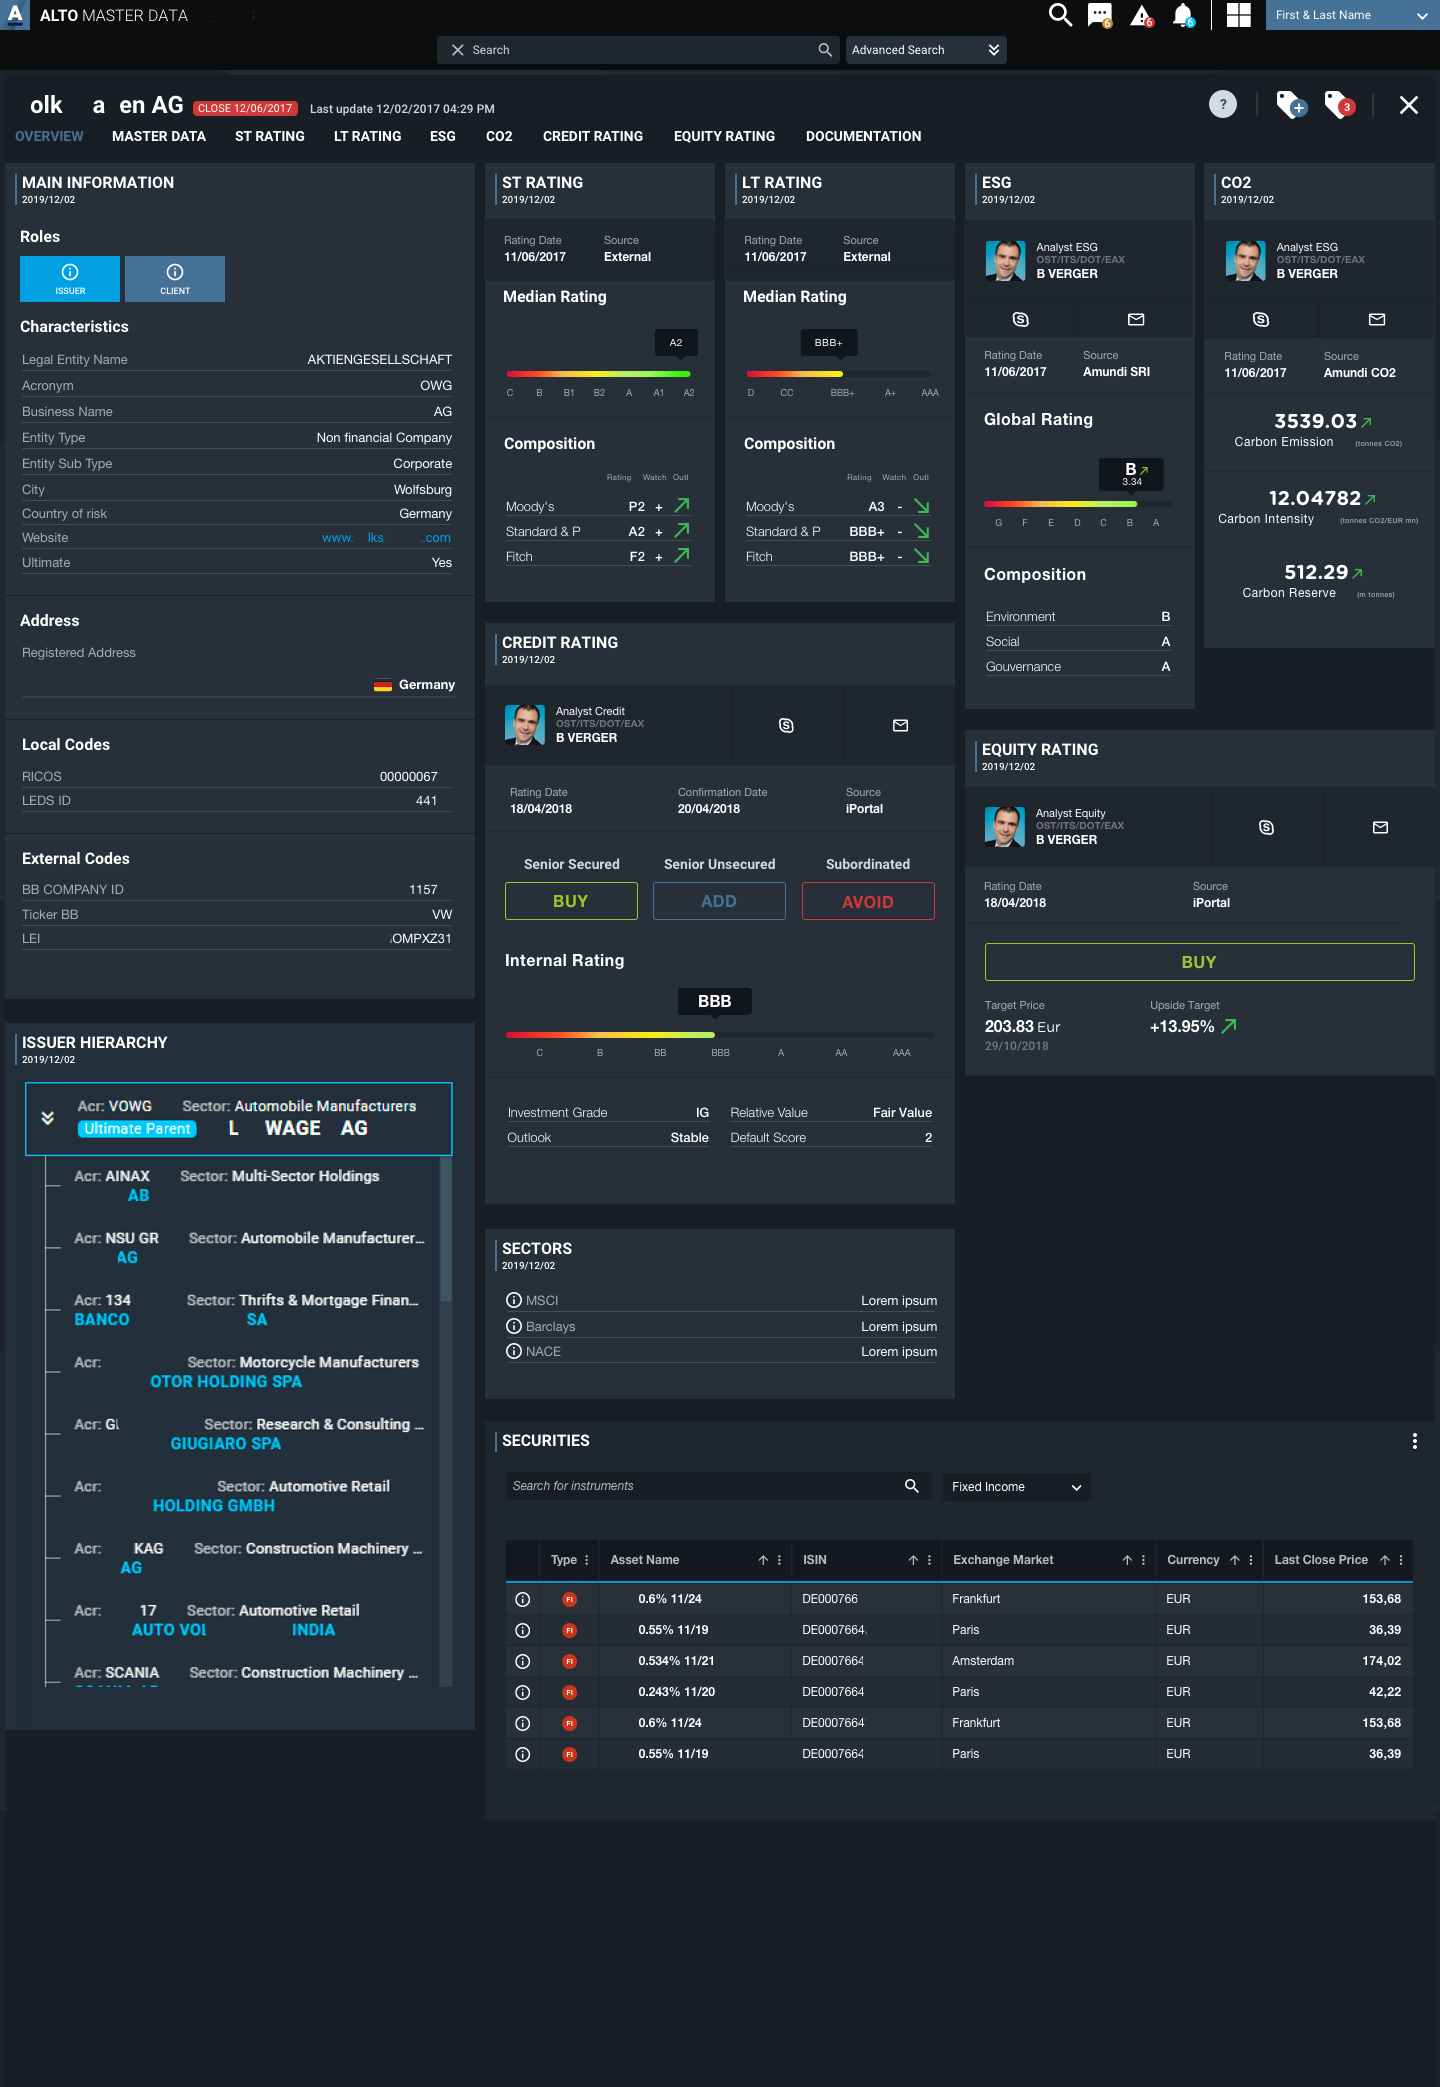
\includegraphics[width=\columnwidth]{img/invisionEx.png}
    \caption{Résultat attendu depuis Invision}
    \label{fig:altoInv}
\end{figure}
\begin{figure}[ht]
    \centering
    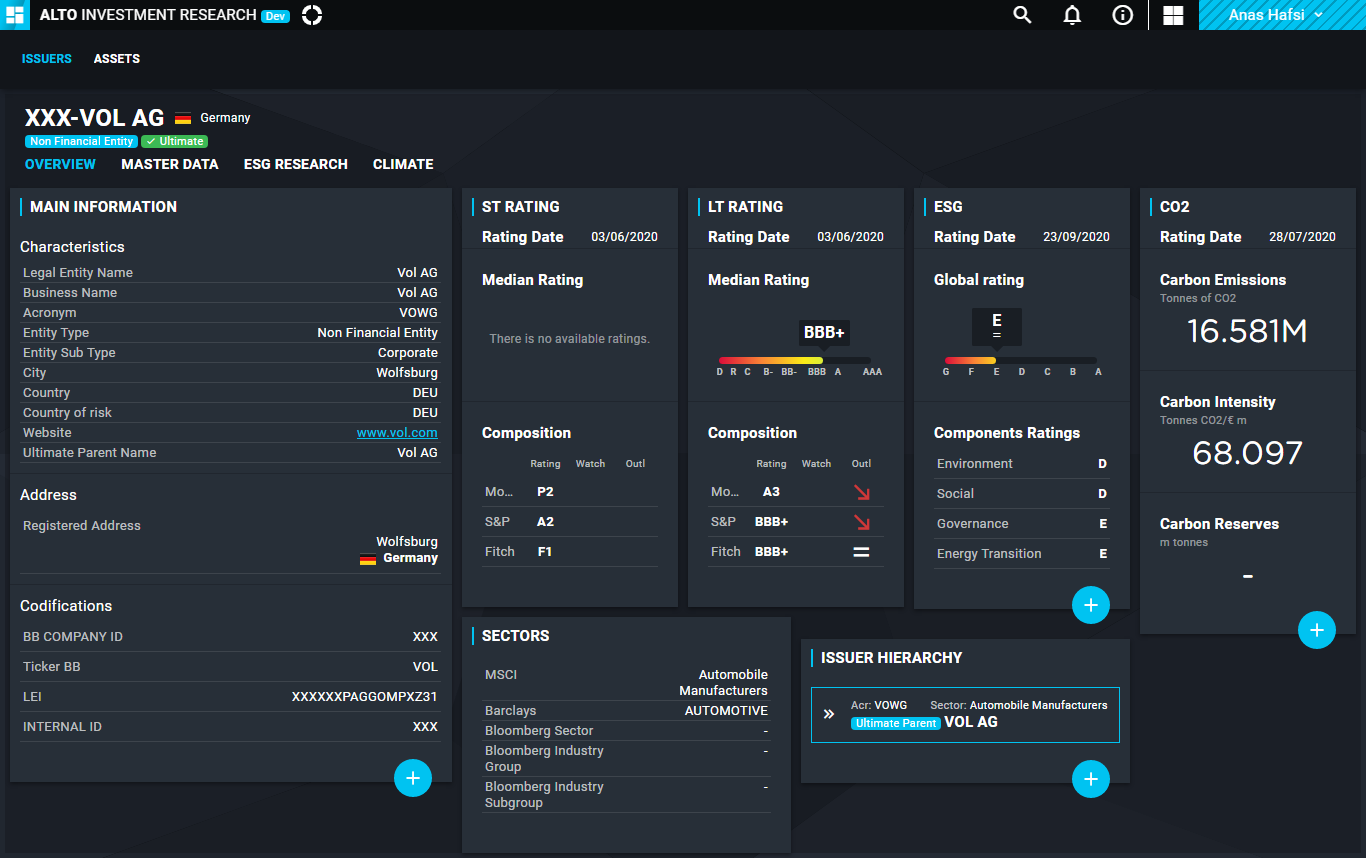
\includegraphics[width=\columnwidth]{img/investmentRsch.png}
    \caption{Version actuelle d'Alto Investment Research}
    \label{fig:altoCurent}
\end{figure}
\chapter{Conclusion générale}
\par C'est la conclusion